\documentclass[12pt, a4paper]{article}%{{{
\usepackage[utf8]{inputenc}
\usepackage[T1]{fontenc}
\usepackage[a4paper,left=2cm,right=2cm,top=2cm,bottom=2cm]{geometry}
\usepackage[frenchb]{babel}
\usepackage{libertine}
\usepackage{float}
\usepackage{hyperref}
\usepackage{amsfonts}
\usepackage{amssymb}
\usepackage[dvipsnames]{xcolor}
\usepackage[pdftex]{graphicx}

\setlength{\parindent}{0cm}
\setlength{\parskip}{1ex plus 0.5ex minus 0.2ex}
\newcommand{\hsp}{\hspace{20pt}}
\newcommand{\HRule}{\rule{\linewidth}{0.5mm}}

\begin{document}

\begin{titlepage}
  \begin{sffamily}
  \begin{center}

    % Upper part of the page. The '~' is needed because \\
    % only works if a paragraph has started.
    
\includegraphics[scale=1]{Images/polytechnique_genie_gauche_fr_rgb.png}~\\[1.5cm]

    \textsc{\LARGE École Polytechnique Montréal}\\[2cm]

    \textsc{\Large INF8405 : Informatique Mobile}\\[1.5cm]

    % Title
    \HRule \\[0.4cm]
    { \huge \bfseries TP2 : Intégration de Maps\\[0.4cm] }

    \HRule \\[2cm]
    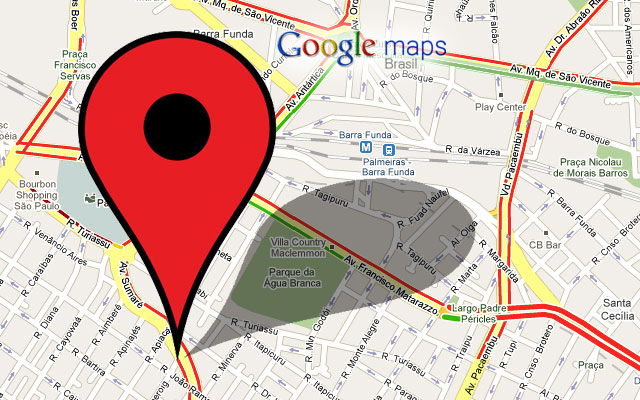
\includegraphics[scale=0.3]{Images/Google-Maps.jpg}\\[2cm]

    % Author and supervisor
    \begin{minipage}{0.4\textwidth}
      \begin{flushleft} \large
          Philippe TROCLET \textsc{1815208}\\
          Alexandre  MAO \textsc{1813566}\\
          Fabien  BERQUEZ \textsc{1800325}\\
      \end{flushleft}
    \end{minipage}
    \begin{minipage}{0.4\textwidth}
      \begin{flushright} \large
        \emph{Soumis à :} M. Aurel Josas RANDOLF\\
        \emph{Soumis le :} 23 Mars 2016  \\
        \emph{Session} Hiver 2016 
      \end{flushright}
    \end{minipage}

    \vfill

  \end{center}
  \end{sffamily}
\end{titlepage}%}}}


\section{Introduction}
L'objectif du TP n°2 était de développer une application destinée à faciliter les rencontres entre membres d'un groupe. Plus précisément, les requis de l'application étaient centrés autour de l'utilisation de différentes ressources, comme le GPS, le calendrier des membres, des API externes comme Google Maps ou Google Places. L'application devait permettre à chaque personne du groupe de définir son profil (nom, courriel, lieux de rencontre préférés) et s'il était organisateur ou non. Une fois ceci fait, et le groupe constitué, l'application, en se basant sur les lieux de rencontre préférés et la position géographique des membres du groupe, proposait trois options de rendez-vous. Les membres du groupe devaient alors choisir chacun l'option qui leur convenait le mieux. Le résultat était transmis à l'organisateur qui pouvait alors définir un lieu et une heure, d'après les disponibilités des membres du groupes, ainsi qu'un petit texte présentant le choix qu'il a retenu. Les informations étaient alors transmises à tous les membres du groupe afin que ceux-ci disposent des informations nécessaires pour aller au rendez-vous.\\
D'un point de vue technique, l'application a pour requis d'être exécutable sur les plateformes Android supportant l'API 18 et supérieures (jusqu'à la version 23 pour la plus récente), c'est à dire des versions d'Android 4.3 à Android 6.0. L'application doit être capable d'être utilisable, avec des fonctionnalités réduites, même lorsque la connexion au réseau cellulaire ou Wi-Fi n'est pas possible, ce qui a eu un impact sur les choix d'implémentation réalisés lors du développement de cette application.  


\section{Présentation générale}
Une première fonctionalité, qui nous semblait importante est la capacité de s'authentifier sur n'importe quel mobile. C'est-à-dire
que l'utilisateur peut posséder  plusieurs appareils mobiles (plusieurs portables ou encore un portable et un tablette), et il
pourra s'authentifier avec le même compte sur tous ces appareils. L'utilisateur peut, sur la page de login, s'identifier va un
motde passe et l'adresse mail associée à son compte. Lors de la création du compte, ses derniers sont stockés sur le serveur.
Au moment du login, on interroge la base de données pour savoir si le mot de passe rentré par l'utilisateur est bien celui qui est
associé à ce compte. Si l'utilisateur utilise un nouvel appareil, ses données seront téléchargées depuis le serveur.
\newline

Il est également possible de créer, sur la page associée au groupe, un nouveau groupe et de le sauvegarder sur le serveur. Ce
serveur contient toutes les données relatives aux utilisateurs est aux groupes. Cela permet potentiellement à chaque utilisateur
de récupérer les préférences de tous les autres et donc d'organiser des rencontres en fonction des préférences de chacun.
\newline

Afin, dans une certaine mesure, de permettre le fonctionnement hors-ligne, une base de données sql lite est également présente.
Elle permet de récupérer les données des autrres utilisateurs afin de potentiellement consulter leur profil ou encore la fiche de
description des groupes. De même, elle permettrait de consulter les événements déjà prévus pour un groupe, ainsi que de consulter
leur description (si celle-ci a été rentrée). Cette fonctionnalité permettrait de mieux se préparer pour les événements à venir.


\section{Présentation Technique}
    \subsection{Partie Serveur}
    Les différents utilisateurs doivent communiquer entre eux afin de pouvoir voter, mais aussi pour connaître la position de chacun
des utilisateurs. Une telle communication nécessite la présence d'un serveur connu de tous. Pour mettre en place une serveur nous
avons choisi d'utiliser le service cloud \textit{firebase}. Les données sont stockées sous le format jason sur le serveur. On peut
alors les récupérer via leur id (générés par l'API firebase).
\newline

Cette solution a plusieurs avantages:
\begin{enumerate}
    \item la présence d'une API déjà testée et éprouvée, ce qui limite le nombre de bugs. Et permet de ne pas réinventer la roue.
    \item la présence de mécanismes de pour écouter des données sur le serveur et être informé en cas de modification.
    \item une grande communauté d'utilisateurs, ce qui facilite la recherche d'information en cas de débogguage.
\end{enumerate}

Ainsi, les coordonnées (longitude/latitude) de chaque utilisateur peuvent être mises à jour sur le serveur en temps réel (ou
presque). Il suffit pour cela d'envoyer ces nouvelles coordonnées sur le serveur à chaque fois que la \textit{callback} associée
au changement de position dans \textit{maps} est appelée. (L'envoie se ferait dans la dite \textit{callback}). Les autres membres
du groupe n'aurait qu'à écouter ces coordonnées sur le serveur afin d'être informé de tous changements de position.
\newline

Cette approche est un peu gourmande en terme de réseau, aussi il est possible de mettre à jour les données que à des moments jugés
opportuns. On obtient alors une meilleure utilisation du réseau mais on perd le temps réel.

    \subsection{Gestion de la Base de données SQL}
    Si la partie serveur utilise Firebase pour stocker les différentes données, il a fallu réfléchir à un moyen alternatif de disposer des dernières données à jour en local, sur l'appareil mobile de l'utilisateur, au cas où celui ci ne disposerait pas d'une connexion Internet à un moment donné de son utilisation de l'application. Nous avons opté pour une solution commune à ce problème sous Android, à savoir l'existence d'une base de données SQLite sur l'appareil. \\
On peut notablement remarquer que la majorité des objets encapsulant les données de notre application sont doublés d'une autre classe gérant la table associée à ces objets dans la base de données SQLite utilisée. Ces classes ont pour objectifs, entre autres, la définition des tables, la définition des requêtes de récupération, d'insertion et de mise-à-jour des données contenues, ainsi que de créer les objets associés pour les récupérer sous une forme plus adaptée à nos besoins.\\
Lors de la conception de ces bases de données, il est important de noter quelques points pris particulièrement en compte :
\begin{itemize}
\item La création de colonnes numériques destinées à être des identifiants pour lier les éléments de différentes tables et permettre plus facilement de rattacher les éléments allant ensemble dans chacune des tables. On peut noter par exemple que la table Groupe réfère les utilisateurs en faisant partie par leur user_id, ce qui permet de réaliser des jointures et récupérer en une seule requête les informations sur les différents membres d'un même groupe.
\item Cette base de données doit nous permettre de représenter fidèlement le dernier état connu de la base de données en ligne. Elle est donc mise à jour régulièrement et permet de réaliser de manière assez transparente les traitements que nous voulons effectuer à un moment donnée, que la base de données en ligne soit accessible ou non.
\end{itemize}
\section{Difficultés rencontrées}
    Comme tous les projets intéressants, celui-ci n'a pas été sans écueils. Ce projet comporte de nombreuses facettes, il doit
posséder une base de données internes, un serveur et pouvoir communiquer avec les API google afin de récupérer des données sur la
position de l'utilisateur courant et sur les lieux (cafés, restaurants, bars) proches d'une certaine position. Il y a donc des
domaines différents à explorer. Le plus simple est alors de répartir ces domaines entre les membres du groupe. Mais s'il chacun
travaille trop de son côté, il devient compliquer d'intégrer les différents travaux respectifs. Le problème est donc avant tout un
problème de communication.
\newline

Cette difficulté est d'autant plus accentuée que ces facettes ne sont pas indépendantes: la base de données doit connaître les
positions afin d'informer les autres utilisateurs lorsqu'ils en font la demande. De ce fait, Les différentes facettes seront très
liées. Et leurs codes respectifs vont, à terme, s'entrecroiser. Ce qui rend leur intégration beaucoup plus compliquée.

\newline
Un autre problème rencontré a été beaucoup plus contraignant, car il a impacté fortement notre travail et nous en a même fait perdre une partie non négligeable (environ une journée de travail). Il s'agit du dépôt Git utilisé, qui a rencontré un problème majeur nous ayant fait perdre les derniers commits réalisés au cours d'une journée relativement chargée. Alexandre a notamment été fortement handicapé par ce problème car il disposait des dernières versions testées des classes traitant de la base de données. Le retard accumulé dans ce domaine a fini par se répercuter sur le développement d'autres fonctionnalités qui se retrouvaient en suspens, car dépendantes de la présence d'une base de données locales fonctionnelle. Nous avons essayé au maximum de limiter les dommages occasionnés sur notre travail, mais la marge de temps était assez restreinte. Certaines fonctionnalités des requis en ont probablement pâti. 
\section{Critiques et suggestions}
    \subsection{Critiques}
    La principale critique que nous avons quant à ce projet réside dans la suggestion d'utiliser \textit{Google Drive} comme serveur. Ce service n'est pas approprié pour un tel usage. L'API Android ne permet tout simplement pas de récupérer des fichiers qui
ont été créés par le programme faisant appel à l'API. De plus, le partage des fichiers entre différents utilisateurs est
laborieux. Et l'utiliser comme serveur demanderait  de réimplémenter de nombreux mécanismes. en particulier il faudrait
réimplémenter des mécanismes d'écoute et de mise à jour. De nombreuses alternatives gratuites existent, il est donc dommage de
proposer \textit{Google Drive}. Il serait, à notre sens, préférable de ne rien indiquer et de laisser aux étudiants le soin de
rechercher leur propre solution.

    \subsection{Suggestions}
    \input{suggestions.tex}
\end{document}
